\documentclass[../main.tex]{subfiles}

\begin{document}

\begin{figure}[h]
    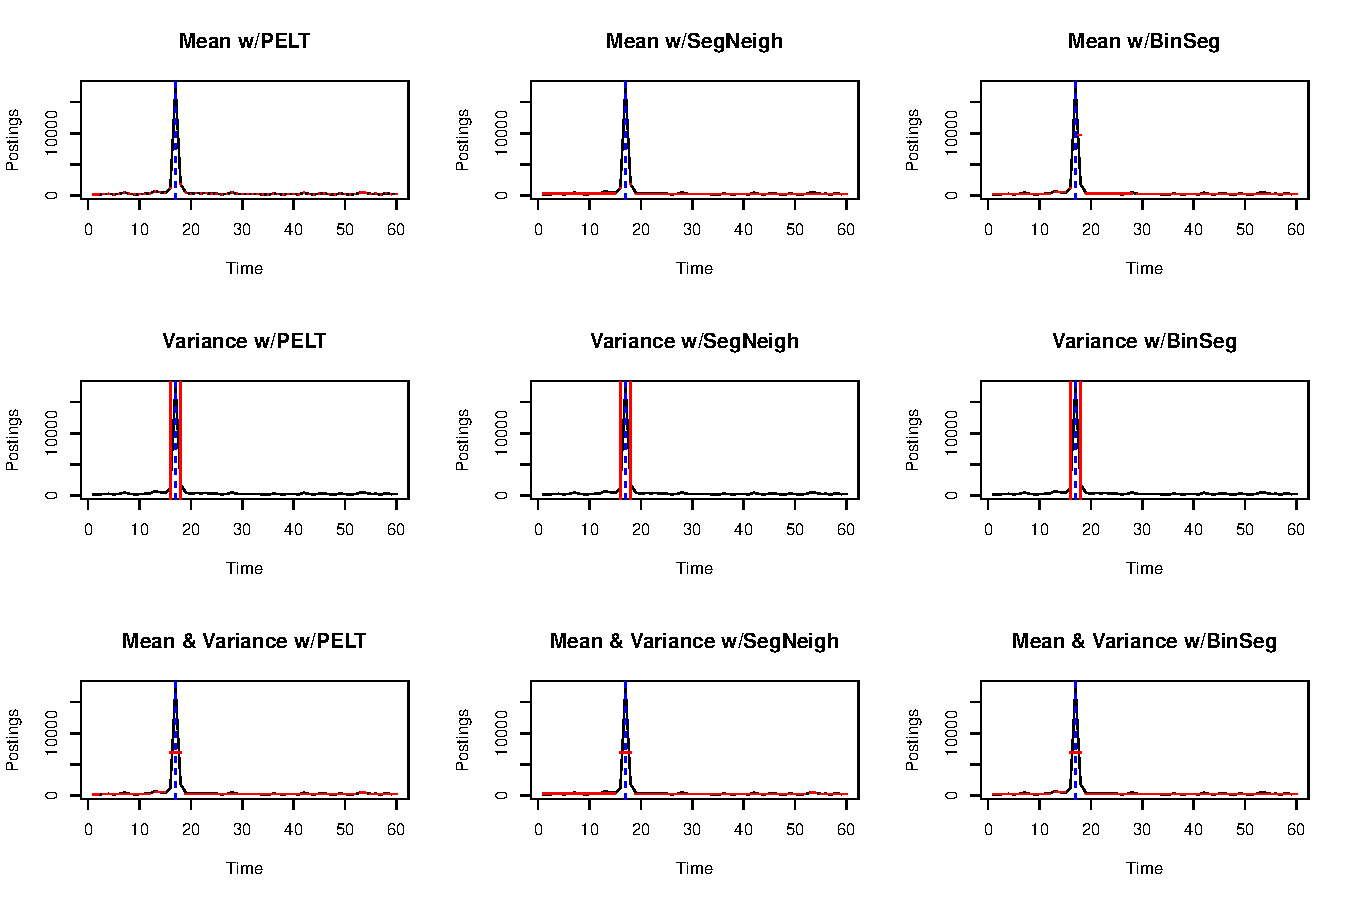
\includegraphics[width=\textwidth]{figures/dirkresults}
    \caption{`Dirk' Change Point Detections}
    \label{fig:dirk}
\end{figure}

\begin{figure}[h]
    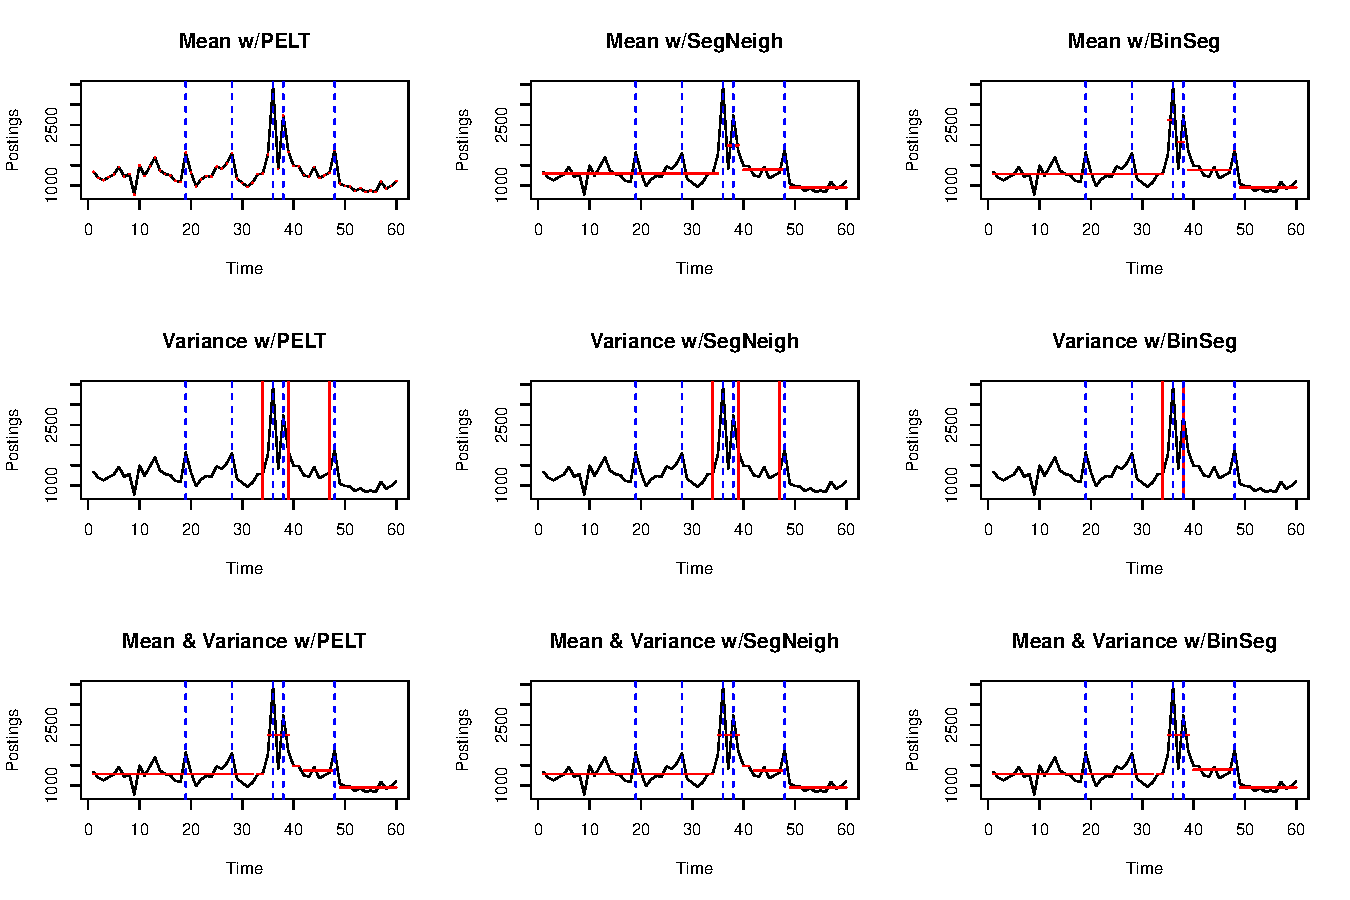
\includegraphics[width=\textwidth]{figures/ziggoresults}
    \caption{`Dirk' Change Point Detections}
    \label{fig:ziggo}
\end{figure}


\begin{figure}[h]
    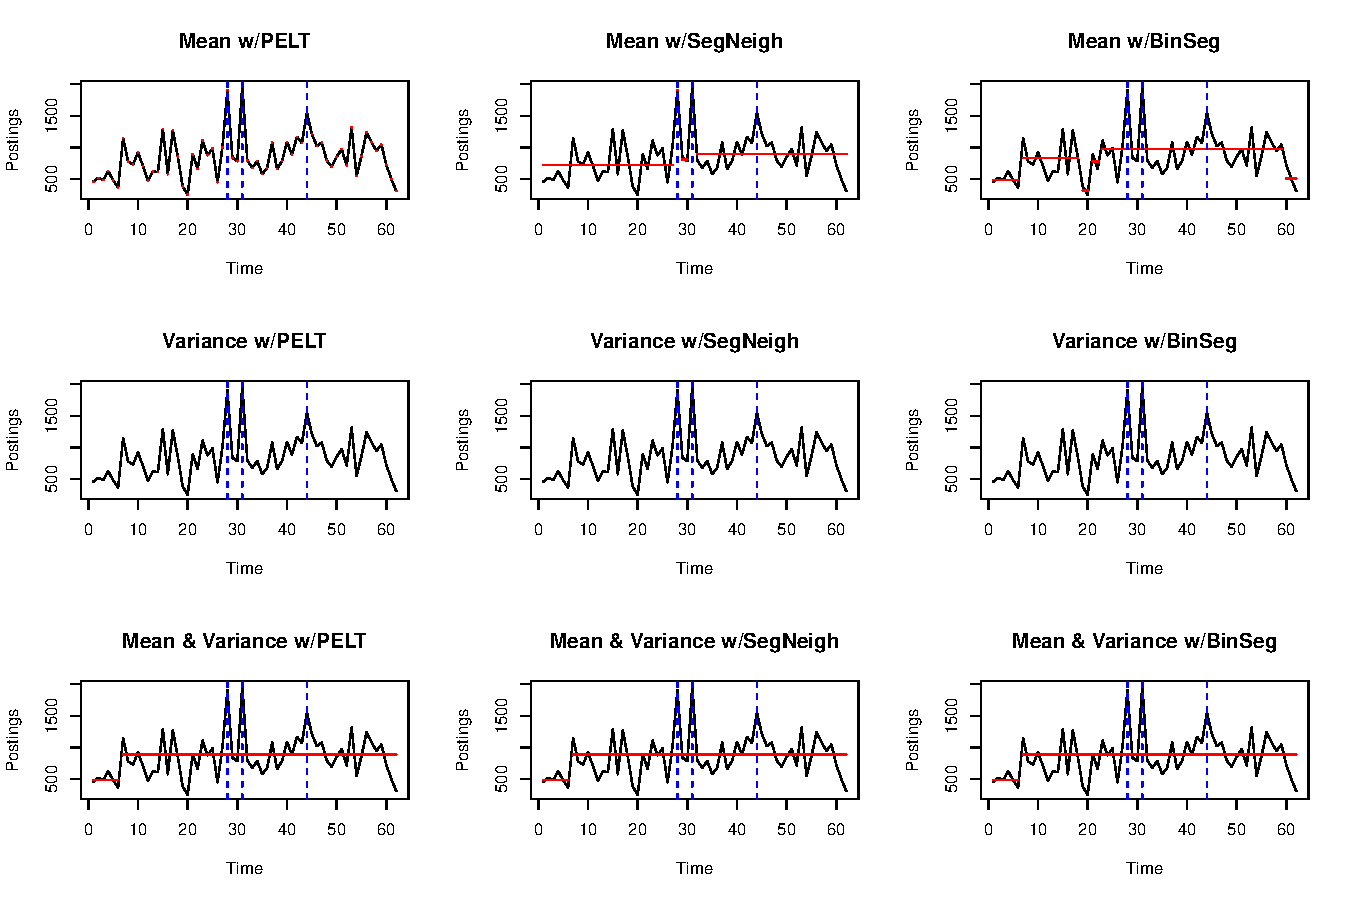
\includegraphics[width=\textwidth]{figures/bolresults}
    \caption{`Dirk' Change Point Detections}
    \label{fig:bol}
\end{figure}


\begin{figure}[h]
    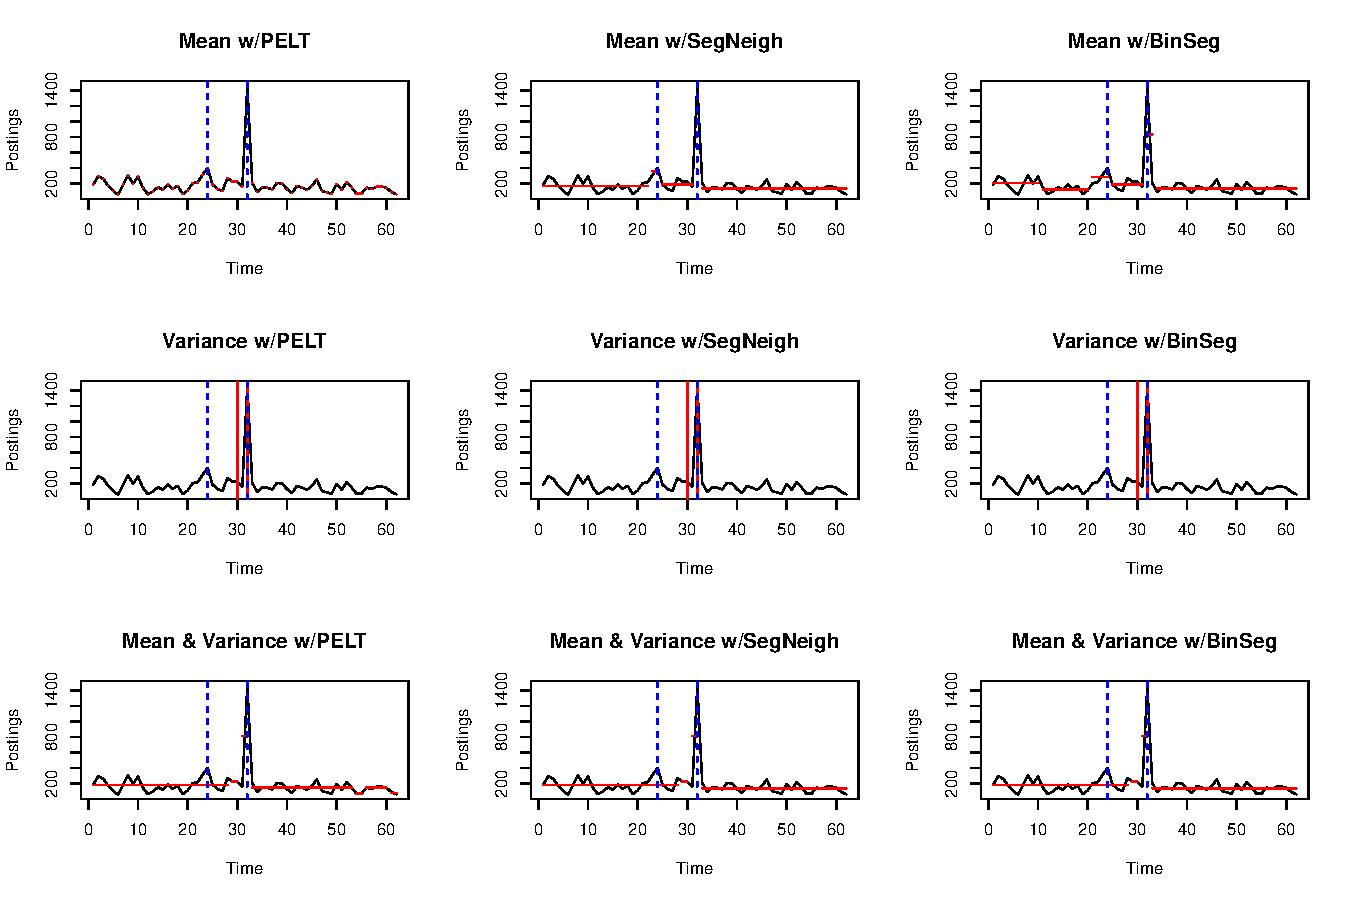
\includegraphics[width=\textwidth]{figures/connexxionresults}
    \caption{`Dirk' Change Point Detections}
    \label{fig:connexxion}
\end{figure}

\begin{figure}[h]
    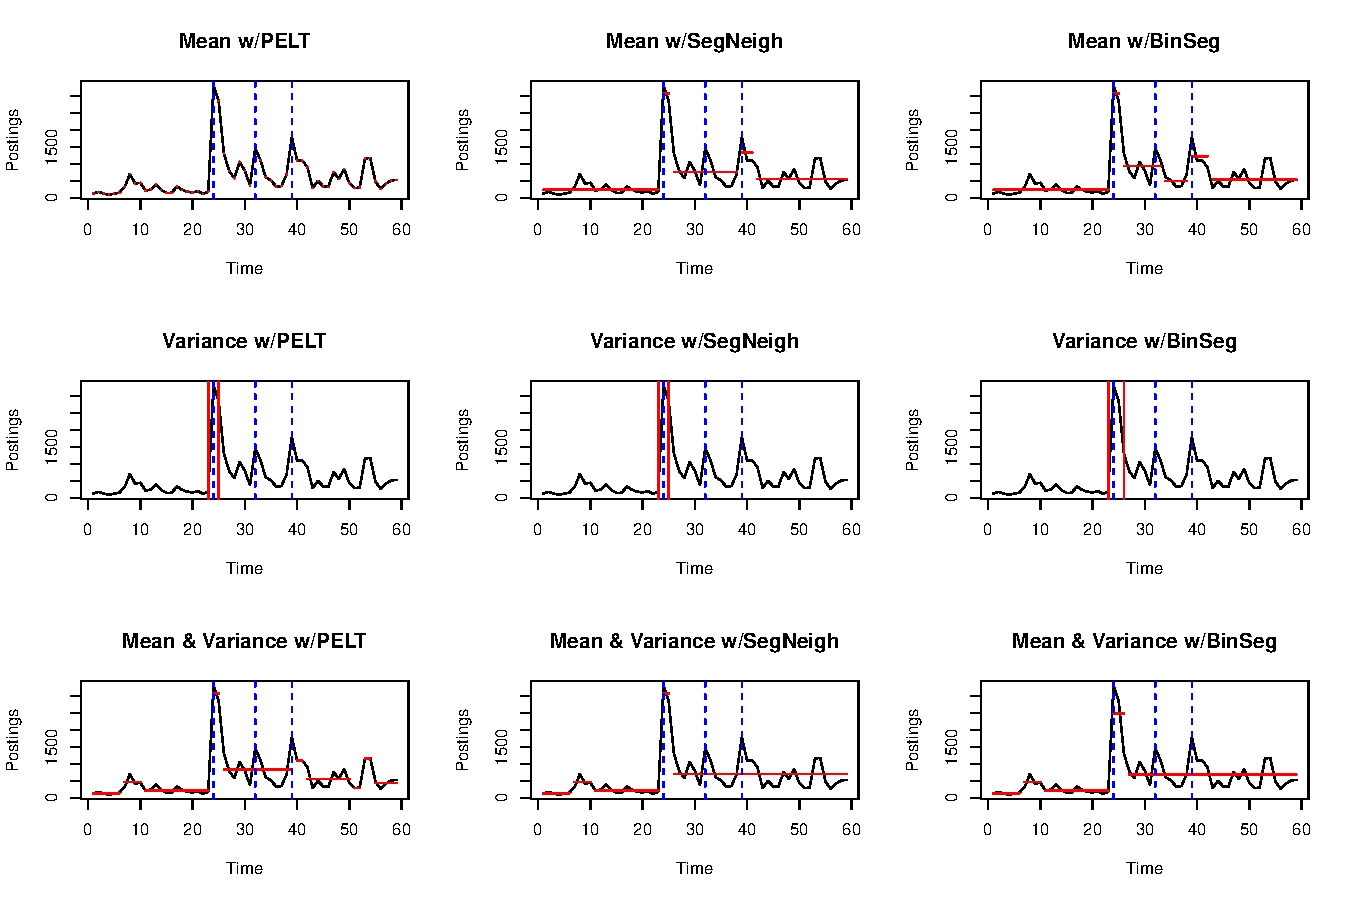
\includegraphics[width=\textwidth]{figures/dapresults}
    \caption{`Dirk' Change Point Detections}
    \label{fig:dap}
\end{figure}

\begin{figure}[h]
    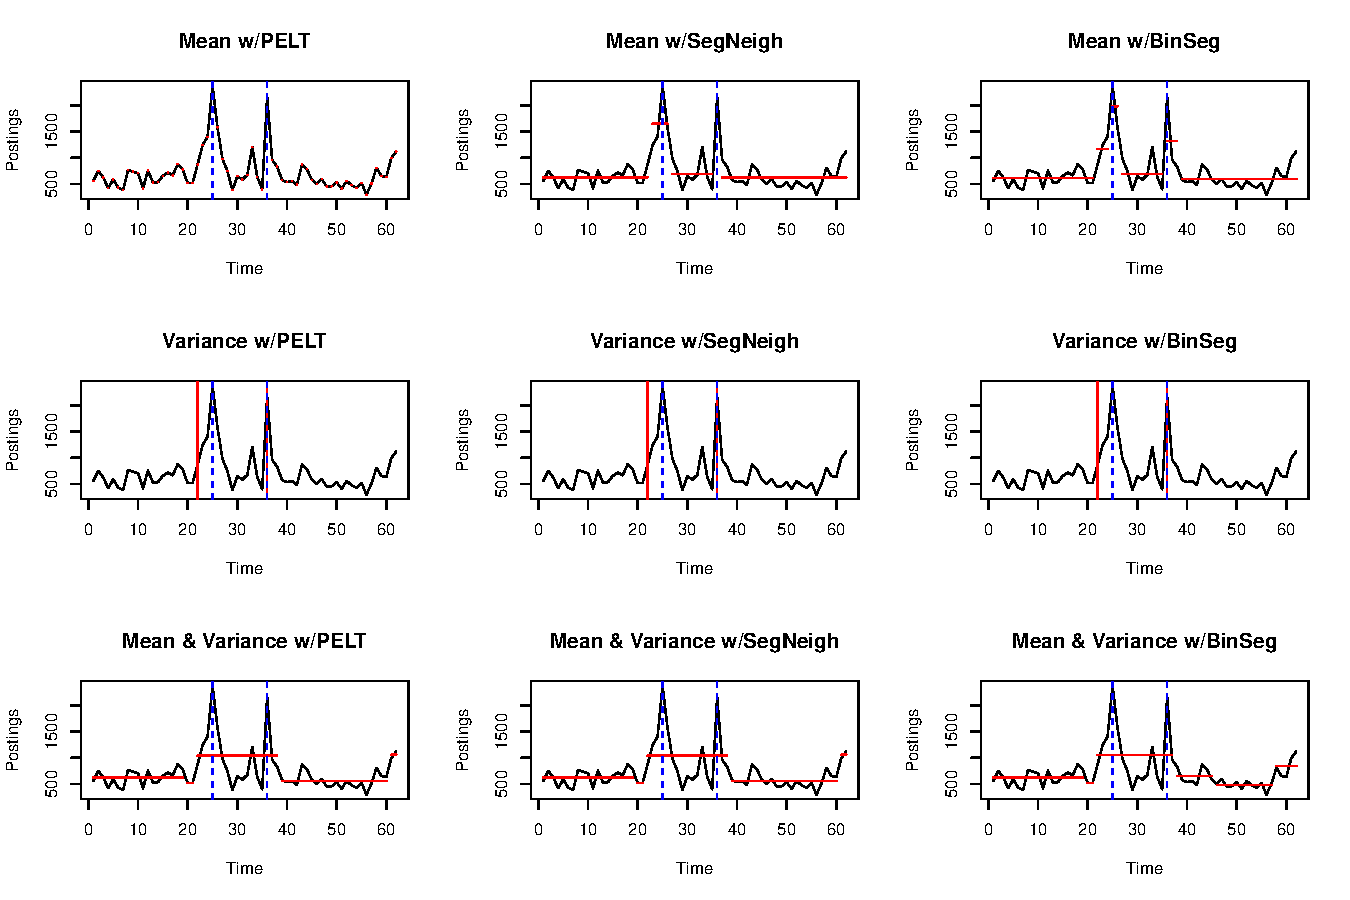
\includegraphics[width=\textwidth]{figures/jumboresults}
    \caption{`Dirk' Change Point Detections}
    \label{fig:jumbo}
\end{figure}

\begin{figure}[h]
    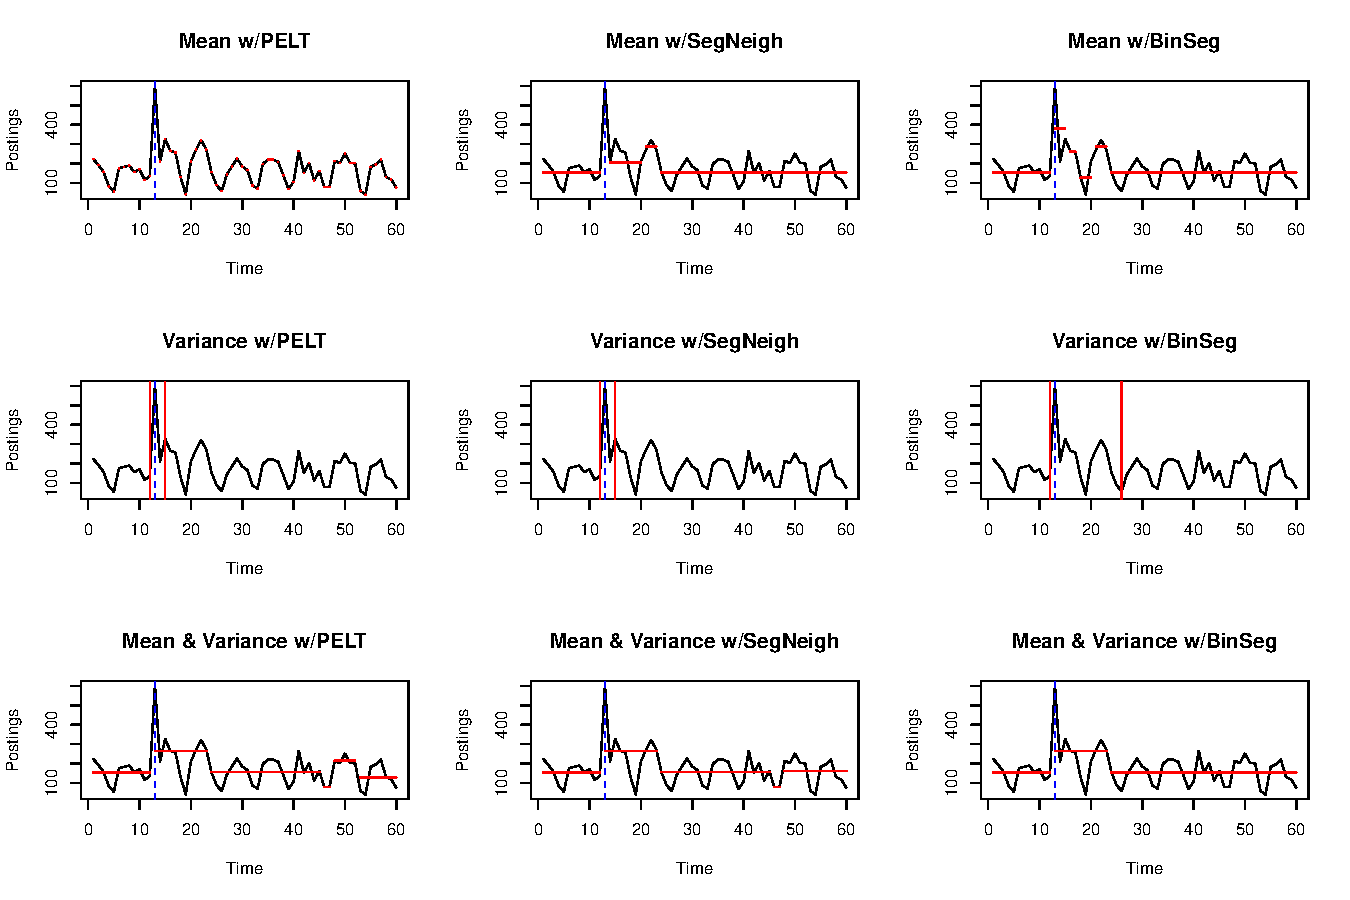
\includegraphics[width=\textwidth]{figures/kvkresults}
    \caption{`Dirk' Change Point Detections}
    \label{fig:kvk}
\end{figure}

\begin{figure}[h]
    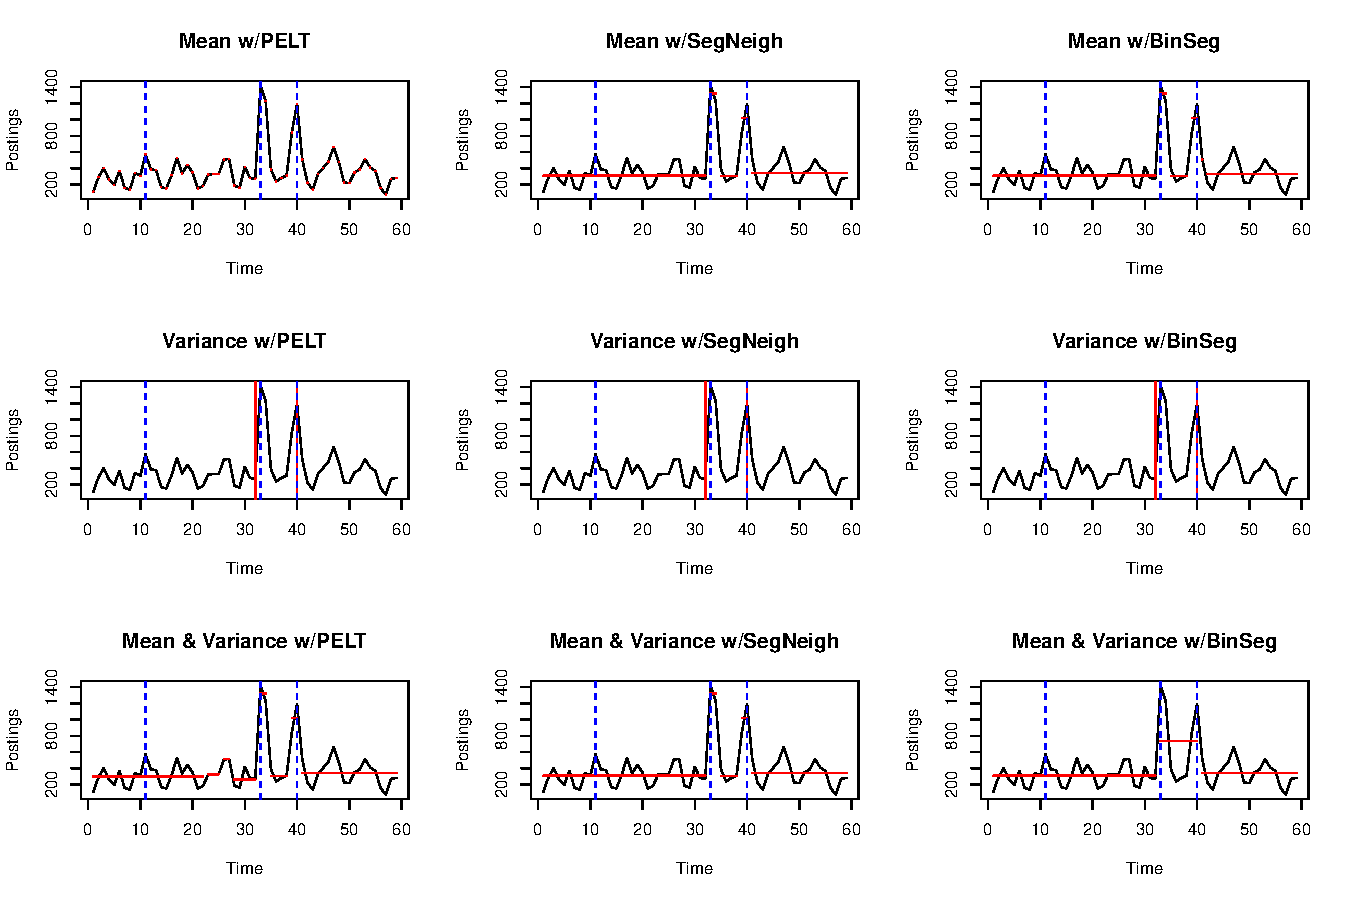
\includegraphics[width=\textwidth]{figures/rabobankresults}
    \caption{`Dirk' Change Point Detections}
    \label{fig:rabobank}
\end{figure}


\begin{figure}[h]
    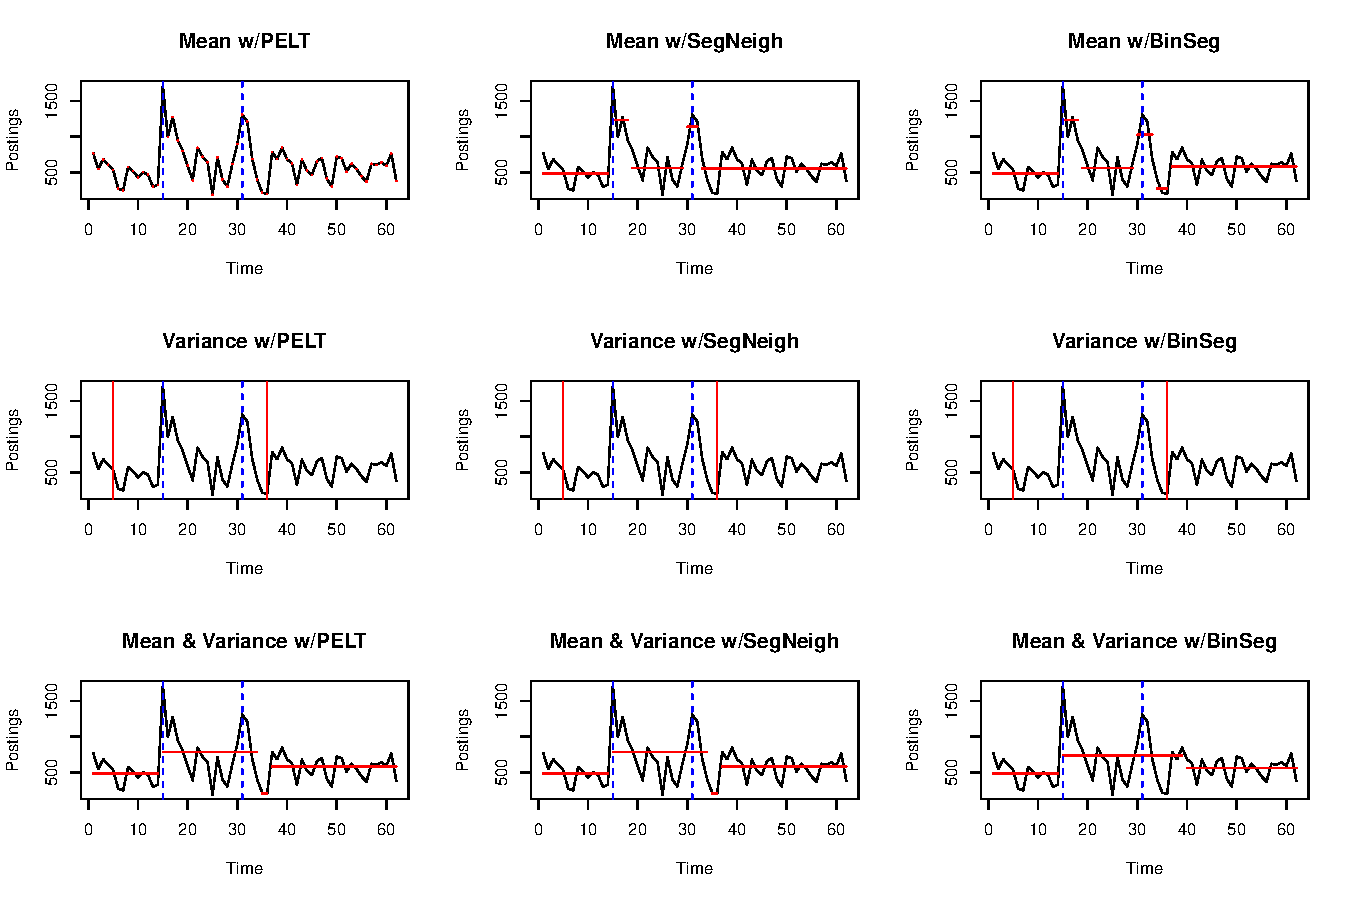
\includegraphics[width=\textwidth]{figures/tele2results}
    \caption{`Dirk' Change Point Detections}
    \label{fig:tele2}
\end{figure}


\begin{figure}[h]
    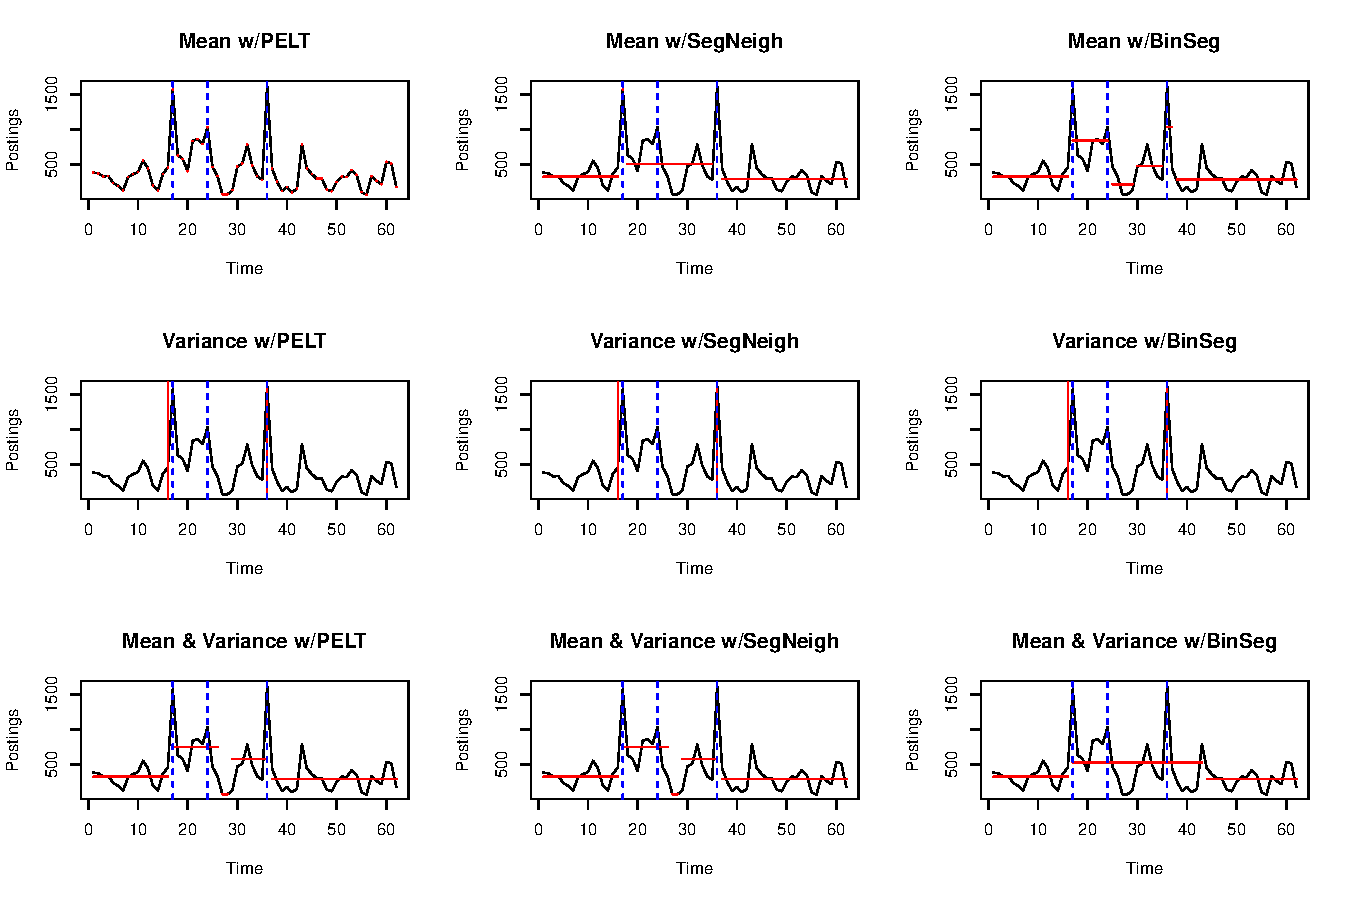
\includegraphics[width=\textwidth]{figures/uwvresults}
    \caption{`Dirk' Change Point Detections}
    \label{fig:uwv}
\end{figure}

\end{document}